\section{Bodediagramm}

Beispiele verschiedener Bodediagramme und zugehötiger Pol-Nullstellen-Diagramme \\
siehe Skript, Kapitel 5.4.3 (S. 222)


\subsection{Bodediagramme mit Matlab}

\lstinputlisting{snippets/bode.m}


\subsection{Approximationen im Bodediagramm}{230}

\subsubsection{Pol im Ursprung}

\begin{minipage}[t]{0.48\columnwidth}
    $$ H(s) = \frac{\alpha}{s} \cbl{= \frac{2}{s}} $$
    \begin{center}
    % Gain
    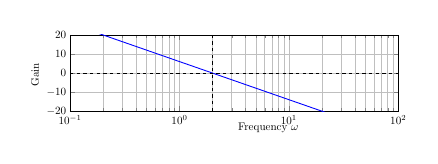
\begin{tikzpicture}
        [
            scale = 0.4,
            >=latex
        ]
        \begin{axis}
            [
                width=12cm,
                height=4cm,
                xmode=log,
                xmin=0.1, xmax=100, ymin=-20, ymax=20,
                x label style={anchor=west},
                xlabel=Frequency $\omega$,
                y label style={anchor=south},
                ylabel=Gain $\deci \bel$,
                xmajorgrids=true,
                xminorgrids=true,
                ymajorgrids=true
            ]

            \addplot[thick, color=blue, domain=0.1:100]{-20*log10(x)+6};

            \addplot[dashed, color=black, domain=0.1:100]{0};
            \addplot[dashed, color=black, domain=2:2] coordinates {(2, -20) (2, 20)};
        \end{axis}
        
    \end{tikzpicture}


    % Phase
    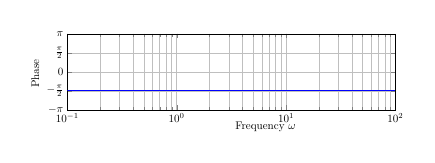
\begin{tikzpicture}
        [
            scale = 0.4,
            >=latex
        ]
        \begin{axis}
            [
                width=12cm,
                height=4cm,
                xmode=log,
                xmin=0.1, xmax=100, ymin=-3.141, ymax=3.141,
                x label style={anchor=west},
                xlabel=Frequency $\omega$,
                y label style={anchor=south},
                ylabel=Phase $\rad$,
                ytick={-3.14, -1.57, 0, 1.57, 3.14},
                yticklabels={$-\pi$, $-\frac{\pi}{2}$, $0$, $\frac{\pi}{2}$, $\pi$},
                xmajorgrids=true,
                xminorgrids=true,
                ymajorgrids=true
            ]
            
            \addplot[thick, color=blue, domain=0.1:100]{-1.57};     

        \end{axis}
            
    \end{tikzpicture}
\end{center}


\end{minipage}
\hfill
\begin{minipage}[t]{0.48\columnwidth}
    \myul{Betrag zeichnen}
        \begin{enumerate}
            \item Waagrechte Gerade fein einzeichnen\\bei $0 \, \deci \bel$
            \item Senkrechte Gerade fein einzeichnen\\bei $\omega = \alpha$
            \item Gerade mit $-20 \, \frac{\deci \bel}{\Dek}$ durch Schnittpunkt der beiden feinen Geraden einzeichnen\\
        \end{enumerate}
    
    \myul{Phase zeichnen}
        \begin{enumerate}
            \item Waagrechte Gerade durch $-\frac{\pi}{2}$
        \end{enumerate}
\end{minipage}


\subsubsection{Nullstelle im Ursprung}

\begin{minipage}[t]{0.48\columnwidth}
    $$ H(s) = \alpha \cdot s \cbl{= 3\cdot s} $$
    \begin{center}
    % Gain
    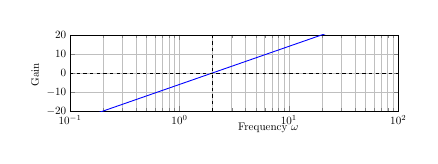
\begin{tikzpicture}
        [
            scale = 0.4,
            >=latex
        ]
        \begin{axis}
            [
                width=12cm,
                height=4cm,
                xmode=log,
                xmin=0.1, xmax=100, ymin=-20, ymax=20,
                x label style={anchor=west},
                xlabel=Frequency $\omega$,
                y label style={anchor=south},
                ylabel=Gain $\deci \bel$,
                xmajorgrids=true,
                xminorgrids=true,
                ymajorgrids=true
            ]

            \addplot[thick, color=blue, domain=0.1:100]{20*log10(x)-6};

            \addplot[dashed, color=black, domain=0.1:100]{0};
            \addplot[dashed, color=black, domain=2:2] coordinates {(2, -20) (2, 20)};
        \end{axis}
        
    \end{tikzpicture}


    % Phase
    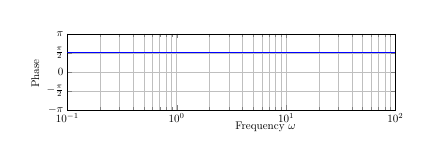
\begin{tikzpicture}
        [
            scale = 0.4,
            >=latex
        ]
        \begin{axis}
            [
                width=12cm,
                height=4cm,
                xmode=log,
                xmin=0.1, xmax=100, ymin=-3.141, ymax=3.141,
                x label style={anchor=west},
                xlabel=Frequency $\omega$,
                y label style={anchor=south},
                ylabel=Phase $\rad$,
                ytick={-3.14, -1.57, 0, 1.57, 3.14},
                yticklabels={$-\pi$, $-\frac{\pi}{2}$, $0$, $\frac{\pi}{2}$, $\pi$},
                xmajorgrids=true,
                xminorgrids=true,
                ymajorgrids=true
            ]
            
            \addplot[thick, color=blue, domain=0.1:100]{1.57};                 
        \end{axis}
            
    \end{tikzpicture}
\end{center}


\end{minipage}
\hfill
\begin{minipage}[t]{0.48\columnwidth}
    \myul{Betrag zeichnen}
        \begin{enumerate}
            \item Waagrechte Gerade fein einzeichnen\\bei $0 \, \deci \bel$
            \item Senkrechte Gerade fein einzeichnen\\bei $\omega = \frac{1}{\alpha}$
            \item Gerade mit $+20 \, \frac{\deci \bel}{\Dek}$ durch Schnittpunkt der beiden feinen Geraden einzeichnen\\
        \end{enumerate}
    
    \myul{Phase zeichnen}
        \begin{enumerate}
            \item Waagrechte Gerade durch $+\frac{\pi}{2}$
        \end{enumerate}
\end{minipage}

\subsubsection{Reeller Pol}

\begin{minipage}[t]{0.48\columnwidth}
    $$ H(s) = \frac{\alpha}{s + \alpha} = \frac{1}{\frac{s}{\alpha} + 1} \cbl{= \frac{4}{s + 4}} $$
    \begin{center}
    % Gain
    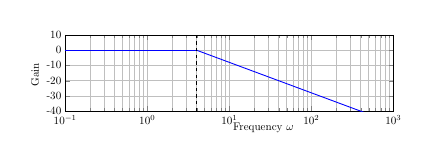
\begin{tikzpicture}
        [
            scale = 0.4,
            >=latex
        ]
        \begin{axis}
            [
                width=12cm,
                height=4cm,
                xmode=log,
                xmin=0.1, xmax=1000, ymin=-40, ymax=10,
                x label style={anchor=west},
                xlabel=Frequency $\omega$,
                y label style={anchor=south},
                ylabel=Gain $\deci \bel$,
                ytick={-40, -30, -20, -10, 0, 10},
                yticklabels={-40, -30, -20, -10, 0, 10},
                xmajorgrids=true,
                xminorgrids=true,
                ymajorgrids=true
            ]

            \addplot[thick, color=blue, domain=0.1:4]{0};  
            \addplot[thick, color=blue, domain=4:1000]{-20*log10(x)+12};   
            
            \addplot[dashed, color=black, domain=4:4]coordinates {(4, -40) (4, 10)};  
        \end{axis}
        
    \end{tikzpicture}


    % Phase
    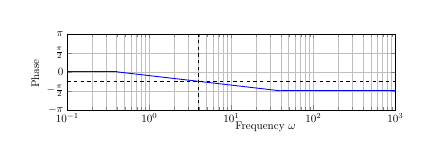
\begin{tikzpicture}
        [
            scale = 0.4,
            >=latex
        ]
        \begin{axis}
            [
                width=12cm,
                height=4cm,
                xmode=log,
                xmin=0.1, xmax=1000, ymin=-3.141, ymax=3.141,
                x label style={anchor=west},
                xlabel=Frequency $\omega$,
                y label style={anchor=south},
                ylabel=Phase $\rad$,
                ytick={-3.14, -1.57, 0, 1.57, 3.14},
                yticklabels={$-\pi$, $-\frac{\pi}{2}$, $0$, $\frac{\pi}{2}$, $\pi$},
                xmajorgrids=true,
                xminorgrids=true,
                ymajorgrids=true
            ]
            
            \addplot[thick, color=blue, domain=0.1:0.4]{0};  
            \addplot[thick, color=blue] coordinates{(0.4, 0) (40, -1.57)};   
            \addplot[thick, color=blue, domain=40:1000]{-1.57};  
            
            \addplot[dashed, color=black, domain=4:4] coordinates {(4, -3.14) (4, 3.14)};  
            \addplot[dashed, color=black, domain=0.1:1000]{-0.79};  

        \end{axis}
            
    \end{tikzpicture}
\end{center}


\end{minipage}
\hfill
\begin{minipage}[t]{0.48\columnwidth}
    \myul{Betrag zeichnen}
    \begin{enumerate}
        \item 0 $\text{dB}$ von $\omega=0$ bis $\omega=\alpha$
        \item $-20\frac{\deci \bel}{\Dek}$ einzeichnen ab $\omega = \alpha$\\
    \end{enumerate}

    \myul{Phase zeichnen}
    \begin{enumerate}
        \item $0$ bis $\omega = \frac{\alpha}{10}$
        \item $-\frac{\pi}{2}$ ab $\omega = 10\cdot \alpha$
        \item Gerade zwischen beiden Geraden 
        \item ($-\frac{\pi}{4}$ bei $\omega=\alpha$)
    \end{enumerate}

\end{minipage}


\subsubsection{Reelle Nullstelle}

\begin{minipage}[t]{0.48\columnwidth}
    $$ H(s) = \frac{s + \alpha}{\alpha} = \frac{s}{\alpha} + 1 \cbl{= \frac{s + 5}{5}} $$
    \begin{center}
    % Gain
    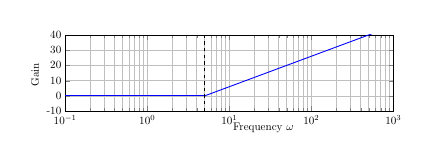
\begin{tikzpicture}
        [
            scale = 0.4,
            >=latex
        ]
        \begin{axis}
            [
                width=12cm,
                height=4cm,
                xmode=log,
                xmin=0.1, xmax=1000, ymin=-10, ymax=40,
                x label style={anchor=west},
                xlabel=Frequency $\omega$,
                y label style={anchor=south},
                ylabel=Gain $\deci \bel$,
                ytick={-10, 0, 10, 20, 30, 40},
                yticklabels={-10, 0, 10, 20, 30, 40},
                xmajorgrids=true,
                xminorgrids=true,
                ymajorgrids=true
            ]

            \addplot[thick, color=blue, domain=0.1:5]{0};  
            \addplot[thick, color=blue, domain=5:1000]{20*log10(x)-14};   
            
            \addplot[dashed, color=black, domain=5:5]coordinates {(5, -10) (5, 40)};  

        \end{axis}
        
    \end{tikzpicture}


    % Phase
    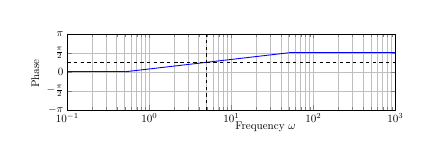
\begin{tikzpicture}
        [
            scale = 0.4,
            >=latex
        ]
        \begin{axis}
            [
                width=12cm,
                height=4cm,
                xmode=log,
                xmin=0.1, xmax=1000, ymin=-3.141, ymax=3.141,
                x label style={anchor=west},
                xlabel=Frequency $\omega$,
                y label style={anchor=south},
                ylabel=Phase $\rad$,
                ytick={-3.14, -1.57, 0, 1.57, 3.14},
                yticklabels={$-\pi$, $-\frac{\pi}{2}$, $0$, $\frac{\pi}{2}$, $\pi$},
                xmajorgrids=true,
                xminorgrids=true,
                ymajorgrids=true
            ]
            
            \addplot[thick, color=blue, domain=0.1:0.5]{0};  
            \addplot[thick, color=blue] coordinates{(0.5, 0) (50, 1.57)};   
            \addplot[thick, color=blue, domain=50:1000]{1.57};  
            
            \addplot[dashed, color=black, domain=5:5] coordinates {(5, -3.14) (5, 3.14)};  
            \addplot[dashed, color=black, domain=0.1:1000]{0.79};                 
        \end{axis}
            
    \end{tikzpicture}
\end{center}
\end{minipage}
\hfill
\begin{minipage}[t]{0.48\columnwidth}

    \myul{Betrag zeichnen}
    \begin{enumerate}
        \item 0 $\text{dB}$ von $\omega=0$ bis $\omega=\alpha$
        \item $+20\frac{\deci \bel}{\Dek}$ einzeichnen ab $\omega = \alpha$\\
    \end{enumerate}

    \myul{Phase zeichnen}
    \begin{enumerate}
        \item $0$ bis $\omega = \frac{\alpha}{10}$
        \item $+\frac{\pi}{2}$ ab $\omega = 10\cdot \alpha$
        \item Gerade zwischen beiden Geraden 
        \item ($+\frac{\pi}{4}$ bei $\omega=\alpha$)
    \end{enumerate}
\end{minipage}
    

\subsubsection{Konjugiert-komplexe Pole}

\begin{minipage}[t]{0.48\columnwidth}
    \raggedright
    \begin{center}
        Voraussetzung: $\abs{q_p} > \frac{1}{2}$
    \end{center}
    $$ H(s) = \frac{\omega_p^2}{s^2 + s \frac{\omega_p}{q_p} + \omega_p^2} \cbl{= \frac{2^2}{s^2 + s \frac{2}{3} + 2^2}} $$

    \begin{center}
    % Gain
    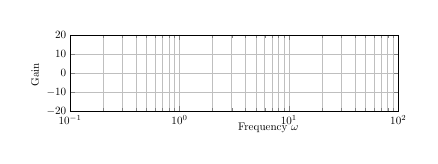
\begin{tikzpicture}
        [
            scale = 0.4,
            >=latex
        ]
        \begin{axis}
            [
                width=12cm,
                height=4cm,
                xmode=log,
                xmin=0.1, xmax=100, ymin=-20, ymax=20,
                x label style={anchor=west},
                xlabel=Frequency $\omega$,
                y label style={anchor=south},
                ylabel=Gain $\deci \bel$,
                xmajorgrids=true,
                xminorgrids=true,
                ymajorgrids=true
            ]

            \addplot[thick, color=blue, domain=0.1:100]{40};
        \end{axis}
        
    \end{tikzpicture}


    % Phase
    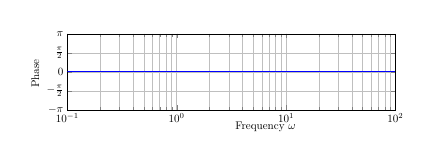
\begin{tikzpicture}
        [
            scale = 0.4,
            >=latex
        ]
        \begin{axis}
            [
                width=12cm,
                height=4cm,
                xmode=log,
                xmin=0.1, xmax=100, ymin=-3.141, ymax=3.141,
                x label style={anchor=west},
                xlabel=Frequency $\omega$,
                y label style={anchor=south},
                ylabel=Phase $\rad$,
                ytick={-3.14, -1.57, 0, 1.57, 3.14},
                yticklabels={$-\pi$, $-\frac{\pi}{2}$, $0$, $\frac{\pi}{2}$, $\pi$},
                xmajorgrids=true,
                xminorgrids=true,
                ymajorgrids=true
            ]
            
            \addplot[thick, color=blue, domain=0.1:100]{0};                 
        \end{axis}
            
    \end{tikzpicture}
\end{center}
\end{minipage}
\hfill
\begin{minipage}[t]{0.48\columnwidth}
    \myul{Betrag zeichnen}
        \begin{enumerate}
            \item 0 $\text{dB}$ von $\omega=0$ bis $\omega=\frac{\omega_p}{2}$
            \item $-40\frac{\text{dB}}{\text{Dek}}$ fein einzeichnen ab $\omega_p$\\
            $\rightarrow$ stark zeichnen ab $\omega = 2 \cdot \omega_p$
            \item Maximalwert $= 20\cdot \log_{10}(q_p)$ bei $\omega_p$
            \item Gerade von $\omega=\frac{\omega_p}{2}$ zu Maximalwert 
            \item Gerade von Maximalwert zu $\omega = 2 \cdot \omega_p$\\
        \end{enumerate}
    \myul{Phase zeichnen}
        \begin{enumerate}
            \item 0 bis $\omega < \frac{\omega_p}{10^{\frac{1}{2 q_p}}}$
            \item $- \pi$ ab $\omega > \omega_p \cdot 10^{\frac{1}{2 q_p}}$
            \item Gerade zwischen $0$ und $\pi$ Geraden
            \item ($- \frac{\pi}{2}$ bei $\omega = \omega_p$)
        \end{enumerate}
\end{minipage}


\subsubsection{Konjugiert-komplexe Nullstellen} 

\begin{minipage}[t]{0.48\columnwidth}
    \raggedright
    \begin{center}
        Voraussetzung: $\abs{q_z} > \frac{1}{2}$
    \end{center}
    $$ H(s) = \frac{s^2 + s \frac{\omega_z}{q_z} + \omega_z^2}{\omega_z^2} \cbl{= \frac{s^2 + s \frac{2}{3} + 2^2}{2^2}} $$

    \begin{center}
    % Gain
    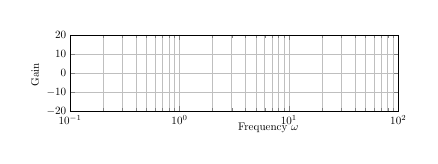
\begin{tikzpicture}
        [
            scale = 0.4,
            >=latex
        ]
        \begin{axis}
            [
                width=12cm,
                height=4cm,
                xmode=log,
                xmin=0.1, xmax=100, ymin=-20, ymax=20,
                x label style={anchor=west},
                xlabel=Frequency $\omega$,
                y label style={anchor=south},
                ylabel=Gain $\deci \bel$,
                xmajorgrids=true,
                xminorgrids=true,
                ymajorgrids=true
            ]

            \addplot[thick, color=blue, domain=0.1:100]{40};
        \end{axis}
        
    \end{tikzpicture}


    % Phase
    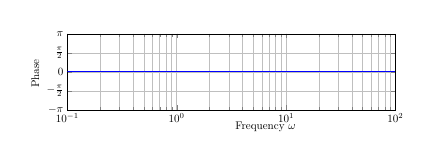
\begin{tikzpicture}
        [
            scale = 0.4,
            >=latex
        ]
        \begin{axis}
            [
                width=12cm,
                height=4cm,
                xmode=log,
                xmin=0.1, xmax=100, ymin=-3.141, ymax=3.141,
                x label style={anchor=west},
                xlabel=Frequency $\omega$,
                y label style={anchor=south},
                ylabel=Phase $\rad$,
                ytick={-3.14, -1.57, 0, 1.57, 3.14},
                yticklabels={$-\pi$, $-\frac{\pi}{2}$, $0$, $\frac{\pi}{2}$, $\pi$},
                xmajorgrids=true,
                xminorgrids=true,
                ymajorgrids=true
            ]
            
            \addplot[thick, color=blue, domain=0.1:100]{0};                 
        \end{axis}
            
    \end{tikzpicture}
\end{center}
\end{minipage}
\hfill
\begin{minipage}[t]{0.48\columnwidth}
    \myul{Betrag zeichnen}
        \begin{enumerate}
            \item 0 $\text{dB}$ von $\omega=0$ bis $\omega=\frac{\omega_z}{2}$
            \item $+40\frac{\text{dB}}{\text{Dek}}$ fein einzeichnen ab $\omega_z$\\
            $\rightarrow$ stark zeichnen ab $\omega = 2 \cdot \omega_z$
            \item Minimalwert $= -20\cdot \log_{10}(q_z)$ bei $\omega_z$
            \item Gerade von $\omega=\frac{\omega_z}{2}$ zu Miniimalwert 
            \item Gerade von Minimalwert zu $\omega = 2 \cdot \omega_z$\\
        \end{enumerate}
    \myul{Phase zeichnen}
        \begin{enumerate}
            \item 0 bis $\omega < \frac{\omega_z}{10^{\frac{1}{2 q_z}}}$
            \item $+ \pi$ ab $\omega > \omega_z \cdot 10^{\frac{1}{2 q_z}}$
            \item Gerade zwischen $0$ und $- \pi$ Geraden
            \item ($\frac{\pi}{2}$ bei $\omega = \omega_z$)\\
        \end{enumerate}
\end{minipage}

\textbf{Hinweis: Berechnungs-Tabelle aus Skript, S. 235} 

\begingroup
\renewcommand{\arraystretch}{2}
\setlength{\tabcolsep}{0mm}
\scalebox{0.33}{
\Huge
\begin{tabularx}{3\columnwidth}{rp{1mm}V{3}*{17}{C}}
    \rowcolor{subsectioncolor!30}$\bm{q_p}$ && $0.5$ & $1$ & $1.5$ & $2$ & $3$ & $4$ & $5$ & $6$ & $8$ & $10$ & $20$ & $50$ & $100$ \\
    \hline
    $\bm{10^{\frac{1}{2 q_p}}}$     && $10$ & $3.16$ & $2.15$ & $1.78$ & $1.47$ & $1.33$ & $1.26$ & $1.21$ & $1.15$ & $1.12$ & $1.06$ & $1.02$ & $1.01$ \\
    \hline
    $\bm{10^{- \frac{1}{2 q_p}}}$   && $0.1$ & $0.316$ & $0.464$ & $0.562$ & $0.681$ & $0.750$ & $0.794$ & $0.825$ & $0.866$ & $0.891$ & $0.944$ & $0.977$ & $0.989$ \\
\end{tabularx}}
\endgroup
\renewcommand{\arraystretch}{1}

\vspace{0.2cm}

% nicht ändern
\begin{minipage}[t]{0.48\columnwidth}
    \raggedright
    \subsubsection{Konstanter Faktor}

    \begin{outline}
        \1 $H(s) = \alpha \cdot e^{\jimg \beta} \cbl{= 3 \cdot e^{\jimg \frac{\pi}{2}}}$
            \2 Betrag $= 20 \cdot \log_{10}(\alpha) = \const$
            \2 Phase $= \beta = \const$
    \end{outline}
    
    \begin{center}
    % Gain
    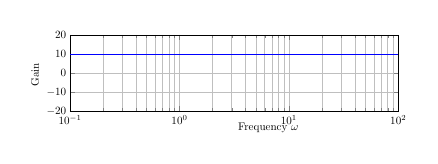
\begin{tikzpicture}
        [
            scale = 0.4,
            >=latex
        ]
        \begin{axis}
            [
                width=12cm,
                height=4cm,
                xmode=log,
                xmin=0.1, xmax=100, ymin=-20, ymax=20,
                x label style={anchor=west},
                xlabel=Frequency $\omega$,
                y label style={anchor=south},
                ylabel=Gain $\deci \bel$,
                xmajorgrids=true,
                xminorgrids=true,
                ymajorgrids=true
            ]

            % K_0
            \addplot[thick, color=blue, domain=0.1:100]{20*log10(3)};
        \end{axis}
        
    \end{tikzpicture}


    % Phase
    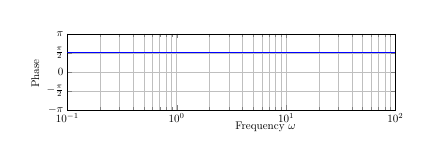
\begin{tikzpicture}
        [
            scale = 0.4,
            >=latex
        ]
        \begin{axis}
            [
                width=12cm,
                height=4cm,
                xmode=log,
                xmin=0.1, xmax=100, ymin=-3.141, ymax=3.141,
                x label style={anchor=west},
                xlabel=Frequency $\omega$,
                y label style={anchor=south},
                ylabel=Phase $\rad$,
                ytick={-3.14, -1.57, 0, 1.57, 3.14},
                yticklabels={$-\pi$, $-\frac{\pi}{2}$, $0$, $\frac{\pi}{2}$, $\pi$},
                xmajorgrids=true,
                xminorgrids=true,
                ymajorgrids=true
            ]
            
            % K_0
            \addplot[thick, color=blue, domain=0.1:100]{1.57};     

        \end{axis}
            
    \end{tikzpicture}
\end{center}
\end{minipage}
\hfill
\begin{minipage}[t]{0.48\columnwidth}
    \raggedright
    \subsubsection{Weitere Bemerkungen}

    \begin{outline}
        \1 \textbf{Inverser Frequenzgang:}
            \2 Amplitudengang an $0 \, \deci \bel$-Linie spiegeln
            \2 Phasengang an $0 \, \rad$- bzw. $0 \, \degree$-Linie spiegeln
        \1 \textbf{Serieschaltung von mehreren Teilsystemen}
            \2 Erfolgt durch \textbf{grafische Addition} der einzelnen Systeme
        \1 Bei Knickpunkten ist Approximationsfehler am grössten
    \end{outline}

\end{minipage}


\subsection{Ergänzung: Konjugiert-komplexe Pole und Nullstellen}{228}

Ein Tiefpass 2. Ordnung enthält eine Überhöhung und somit ein absolutes Maximum. 

$$ \text{UTF Tiefpass 2. Ordnung:} \quad H(s) = \frac{\omega_p^2}{s^2 + s \frac{\omega_p}{q_p} + \omega_p^2} $$

\renewcommand{\arraystretch}{2}
\begin{tabular}{ll}
    Frequenz beim Maximum:  & $ \omega_{\rm max} = \omega_p \cdot \sqrt{1 - \frac{1}{2 q_p^2}} = \sqrt{\omega_p^2 - 2 \sigma_p^2}$ \\
    Höhe des Maximums:      & $ \abs{H(\omega_{\rm max})} = \frac{q_p}{\sqrt{1 - \frac{1}{4 q_p^2}}}$ \\
\end{tabular}

\textrightarrow Es gilt: $\omega_{max} \leq \omega_p$


\subsubsection{Spezialfall $q = 1$}

\renewcommand{\arraystretch}{1.5}
\begin{minipage}[c]{0.55\columnwidth}    
    \begin{tabular}{ll}
        Frequenz:  & $ \omega_{\rm max} = \omega_p \cdot \sqrt{1 - \frac{1}{2}} = \frac{\omega_p}{\sqrt{2}}$ \\
        Höhe:      & $ \abs{H(\omega_{\rm max})} = \frac{1}{\sqrt{1 - \frac{1}{4}}} = 1.15$ \\
    \end{tabular}

\end{minipage}
\hfill
\begin{minipage}[c]{0.43\columnwidth}
    


\begin{tikzpicture}
	[
	x=1cm, y=1cm, scale=0.67, font=\footnotesize, >=latex 
	%Voreinstellung für Pfeilspitzen
	]
	
	%Raster im Hintergrund
	%\draw[step=1, gray!50!white, very thin] (0,0) grid (5.5,1.5);
	
	
	%Länge x Achse
	\draw [-latex] (0,0) -- ++(5.5,0) node[right] {$\omega$};
	
	%Länge y Achse
	\draw [-latex] (0,0) -- ++(0,1.5) node[above] {$\left\lvert H\left(\omega\right) \right\rvert $};
	
	%Zahlen auf y-Achse 
	\foreach \y in {0,1}
	\draw[shift={(0,\y)}] (2pt,0pt) -- (-2pt,0pt);
	
	%Zahlen auf x-Achse
	\foreach \x in {0}
	\draw[shift={(\x,0)},color=black] (0pt,2pt) -- (0pt,-2pt);
	
	%gestrichelte linie
	\draw [dashed, gray, thick] (0,1) -- (4,1);		
	\draw [dashed, orange, thick] (3.2,-0.05) -- (3.2,1.2);
	\draw [dashed, red, thick] (4,-0.05) -- (4,1);
	
	%Beschriftungen
	\draw [] (0,1) node[left] {$1$};
	\draw [] (4,0) node[red, below] {$\omega_p$};	
	\draw [] (3.3,0) node[orange, below] {$\omega_{\rm max}$};
	\draw [] (5.1,0.7) node[] {$-40\frac{\deci \bel}{\text{Dek.}} $};

	%Geschwungene Linie
	\draw[thick, blue] plot[smooth] coordinates {(0,1) (2,1.15) (3.3,1.2) (4,1) (5.2,0)};
	
	%Punkte
	\fill [orange] (3.2,1.2) circle (0.06cm);
	\fill [red] (4,1) circle (0.06cm);
	
\end{tikzpicture}
\end{minipage}


\subsubsection{Spezialfall $q = \frac{1}{2}$}

\begin{minipage}[c]{0.55\columnwidth}
    \begin{tabular}{ll}
            Frequenz:  & $ \omega_{\rm max} = \omega_p \cdot \sqrt{1 - \frac{1}{2 \big(\frac{1}{2} \big)^2 }}$ \\
                       & $ = \omega_p \cdot \sqrt{1-2} \in \mathbb{C}$ \\
            Höhe:      & $ \abs{H(\omega_{\rm max})} = \infty$ \\   % CHECK: macht das Sinn???
    \end{tabular}
\end{minipage}
\hfill
\begin{minipage}[c]{0.43\columnwidth}
    \begin{tikzpicture}
	[
	x=1cm, y=1cm, scale=0.6, font=\footnotesize, >=latex 
	%Voreinstellung für Pfeilspitzen
	]
	
	%Raster im Hintergrund
	%\draw[step=0.1, gray!50!white, very thin] (0,0) grid (5.5,2.5);
	%\draw[step=1, gray!80!white, thin] (0,0) grid (5.5,2.5);
	
	%Länge x Achse
	\draw [-latex] (0,0) -- ++(5.5,0) node[right] {$\omega$};
	
	%Länge y Achse
	\draw [-latex] (0,0) -- ++(0,2.5) node[above] {$\left\lvert H\left(\omega\right) \right\rvert $};
	
	%Zahlen auf y-Achse 
	\foreach \y in {0,1,2}
	\draw[shift={(0,\y)}] (2pt,0pt) -- (-2pt,0pt);
	
	%Zahlen auf x-Achse
	\foreach \x in {0}
	\draw[shift={(\x,0)},color=black] (0pt,2pt) -- (0pt,-2pt);
	
	%gestrichelte linie
	\draw [dashed, gray, thick] (0,1) -- (4,1);		
	\draw [dashed, red, thick] (4,-0.05) -- (4,1);
	
	%Beschriftungen
	\draw [] (0,2) node[left] {$0 \, \deci \bel$};
	\draw [] (0,1) node[left] {$6 \, \deci \bel$};
	\draw [] (4,0) node[red, below] {$\omega_p$};	
	\draw [] (4,1.8) node[] {negative Überhöhung};	

	%Geschwungene Linie
	\draw[thick, blue] plot[smooth] coordinates {(0,2) (1,1.94) (2,1.75) (3,1.44) (4,1) (4.6,0.57) (5.2,0)};
	\draw [-latex, thick] (4,1.6) -- (4,1.1);

	%Punkte

	\fill [red] (4,1) circle (0.06cm);
	
\end{tikzpicture}


\end{minipage}


\subsubsection{Spezialfall $q =\frac{1}{\sqrt{2}}$}

\begin{minipage}[c]{0.55\columnwidth}

    \begin{tabular}{ll}
        Frequenz:   & $ \omega_{\rm max} = 0$ \\
        Höhe:       & $ \abs{H(\omega_{\rm max})} = q_p = \frac{1}{\sqrt{2}}$ \textrightarrow\ $3 \, \deci \bel$ \\
    \end{tabular}
    \renewcommand{\arraystretch}{2}
\end{minipage}
\hfill
\begin{minipage}[c]{0.43\columnwidth}
        

\begin{tikzpicture}
	[
	x=1cm, y=1cm, scale=0.63, font=\footnotesize, >=latex 
	%Voreinstellung für Pfeilspitzen
	]
	
	%Raster im Hintergrund
	%\draw[step=0.1, gray!50!white, very thin] (0,0) grid (5.5,2.5);
	%\draw[step=1, gray!80!white, thin] (0,0) grid (5.5,2.5);
	
	%Länge x Achse
	\draw [-latex] (0,0) -- ++(5.5,0) node[right] {$\omega$};
	
	%Länge y Achse
	\draw [-latex] (0,0) -- ++(0,2.5) node[above] {$\left\lvert H\left(\omega\right) \right\rvert $};
	
	%Zahlen auf y-Achse 
	\foreach \y in {0,1.5}
	\draw[shift={(0,\y)}] (2pt,0pt) -- (-2pt,0pt);
	\foreach \y in {2}
	\draw[shift={(0,\y)}] (2pt,0pt) -- (-2pt,0pt);
	
	%Zahlen auf x-Achse
	\foreach \x in {0}
	\draw[shift={(\x,0)},color=black] (0pt,2pt) -- (0pt,-2pt);
	
	%gestrichelte linie
	\draw [dashed, gray, thick] (0,1.5) -- (4,1.5);		
	\draw [dashed, red, thick] (4,-0.05) -- (4,1.5);
	
	%Beschriftungen
	\draw [] (0,2) node[left] {$0 \, \deci \bel$};
	\draw [] (0,1.5) node[left] {$3 \, \deci \bel$};
	\draw [] (4,0) node[red, below] {$\omega_p$};	
	\draw [] (2,2.3) node[] {maximal flach};	

	%Geschwungene Linie
	\draw[thick, blue] plot[smooth] coordinates {(0,2) (1,1.95) (2,1.85) (3,1.7) (4,1.5) (4.7,1.24) (5.4,0.9)};
	
	\draw [-latex, thick] (1,2.25) -- (0.1,2.05);

	%Punkte
	\fill [red] (4,1.5) circle (0.06cm);
	
\end{tikzpicture}


\end{minipage}
\renewcommand{\arraystretch}{1}